\section{Introducere}

BigchainDB este tehnologia folosită pentru a răspunde nevoilor date de aplicația TrustNews, reușind să facă trecerea ușoară către noile moduri de procesare și stocare a datelor.\\

Tehnologia, ajunsă acum la versiunea 2.0, combină proprietățile blockchain (descentralizare, imutabilitate și management propriu asupra datelor deținute) cu cele ale bazelor de date (rată de tranzacționare mare, timp de răspuns mic și posibilitate de a interoga eficient conținutul). \cite{BigchainDB_Art}\\

\begin{figure}[H] 
\centering
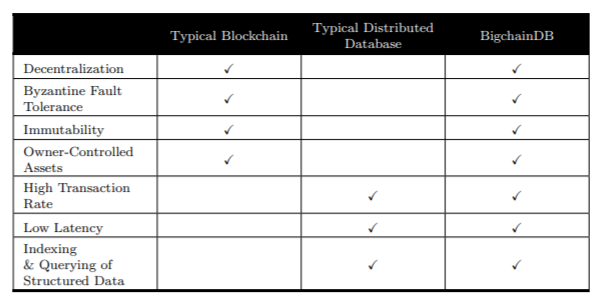
\includegraphics[scale=1]{Images/BCDB_Props.png}
\caption{Proprietăți BigchainDB - sursă: \cite{BigchainDB_Art}}
\end{figure}

\section{Proprietăți}

Structura descentralizată implică noduri deținute și menținute de persoane diferite. Astfel se elimina necesitatea unui singur punct de control sau a unei singure entități care să administreze întreagă rețea.\\

Nodurile sunt compuse din 3 elemente: nucleul Tendermint, server-ul BigchainDB și o bază de date MongoDB. Fiecare contribuie cu elemente specifice pentru a reuni toate proprietățile unui blockchain.\\

\begin{figure}[H] 
\centering
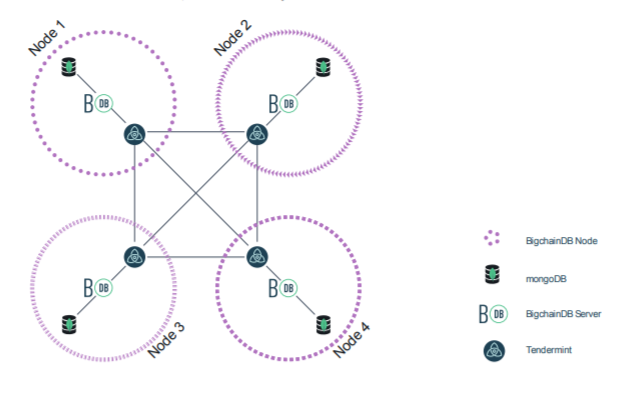
\includegraphics[scale=0.9]{Images/BCDB_Nodes.png}
\caption{Noduri BigchainDB - sursă: \cite{BigchainDB_Art}}
\end{figure}

Tendermint \cite{Tendermint} este tehnologia de bază peste care se lucrează și care aduce elementele ce țin de rețea și de algorimul de consens. Mai exact Tendermint Core este componenta ce permite trimiterea de mesaje în rețea folosind protocoale specifice iar algormitmul de consens este Byzantine Fault Tolerant. Consensul se stabilește pe baza mai multor runde de votare la care participă toate nodurile și în care se decide ce block va fi publicat. Un block este valid dacă pentru fiecare rundă cel puțin două treimi din noduri au votat în favoarea lui.\\

Informația va fi stocată în final în bazele de date de pe fiecare nod. Natura descentralizată oprește atacatorii care ar vrea să corupă sau să șteargă datele. Ei ar putea să obțină privileglii crescute pe anumite noduri însă asta le va permite manipularea datelor doar de pe acele noduri. Încercarea de a acționa rău voit în procesul de votare poate fi nesemnificativ dacă numărul de noduri este unul foarte mare (implicit pragul de două treimi este mare).\\

De menționat este faptul că BigchainDB este deseori într-un context de blockchain cu permisiune. Astfel accesul în rețeaua dezvoltată pentru o anumită aplicație este dat de o autoritate care poate monitoriza acțiunile fiecărui membru și poate lua decizii în consecință.\\

Imposibilitatea de a șterge datele odată salvate în blockchain este realizată practic în software prin lipsa unui serviciu explicit care să permită acest lucru. În plus descentralizarea amintită anterior implică și salvarea în fiecare nod a conținutului din blockchain. Astfel dacă de pe un anumit nod se șterg date, celelalte noduri nu vor fi impactate.\\

Toate bunurile (\textit{assets}) create în BigchainDB aparțin unor anumiți utilizatori. Aceștia pot dovedi posesia lor și le pot transfera atât timp cât pot arată deținerea cheilor criptografice cu care au fost create sau primite structurile de date. Interacțiunea se realizează prin tranzacții specifice de tip CREATE sau de tip TRANSFER descrise în secțiunea următoare. Software-ul se asigură că tranzacțiile sunt valide atât pe partea internă a conținutului cât și la nivel înalt verificând să nu existe situații de double-spending.\\

Rată crescută de tranzacții și timpul de procesare scăzut sunt date de performanța Tendermint. Se asigură timpi de sub o secundă pentru procesarea tranzacțiilor chiar și atunci când vorbim de mii de tranzacții. Trebuie totuși menționat că un scenariu real al conține un minim de 50 de noduri distribuite în mai multe zone geografice ale globului.\\

Indexarea și interogarea datelor se face asupra bazei de date MongoDB. Fiecare nod deține întregul conținutdin blockchain, de la block-uri la elementele particulare din interiorul fiecăruia, sub formă de structuri JSON și este în deplin control asupra propriei clone. Fiecare utilizator poate manevra datele în orice mod dorește și poate crea indexi sau interogări eficiente pentru diferite puncte de interes. Asupra lor se pot adăuga servicii precum apeluri HTTP API pentru a le folosi la o scară largă. De asemenea software-ul BigchainDB aduce câteva modalități predefinite prin care putem extrage informații rapid sub formă de apeluri HTTP API.\\

\clearpage

\section{Utilizare}

BigchainDB pune la dispoziție o serie de utilitare numite drivere cu care putem interacționa cu întregul ecosistem \cite{BigchainDB_Docs}. Există două tipuri, unul scris în Python \cite{BigchainDB_PythonDriver} și unul în JavaScript \cite{BigchainDB_JSDriver} dar rămâne la latitudinea fiecărui utilizator să aleagă cu ce se simte confortabil pentru că ambele au aceleași capacități.\\

La nivel de bază aceste drivere se folosesc de anumite funcții implementate peste componenta din Tendermint numită Application BlockChain Interface (ABCI) \cite{Tendermint_WhatIs}, componentă care permite scrierea de cod ce acționează asupra componentelor blockchain în orice limbaj de programare. BigchainDB definește funcțiile din interfață pentru a putea iniția și finaliza acțiunile de creare a unui block (BeginBlock, EndBlock, Commit) și pentru a valida și trimite tranzacțiile (CheckTx, DeliverTx)\cite{BigchainDB_Art}.\\

Tranzacțiile sunt practic mesajele pe care dorim să le creem, mesaje ce conțin asset-urile pe care dorim să le salvăm în blockchain. \\

Tranzacțiile sunt structuri de tip JSON ce respectă anumite reguli de sintaxă și conținut \cite{BigchainDB_ReadMe}. Sunt compuse din:
\begin{itemize}
    \item \textbf{ID}. Este codul hash SHA-256 calculat pe baza tuturor celorlalte date din tranzacție și reprezintă identificatorul unei tranzacții.
    
    \item \textbf{Versiune}. Reprezintă versiunea de software cu care a fost creată tranzacția și este utilă în preluarea corespunzătoare a regulilor de validare.
    
    \item \textbf{Operație}. Reprezintă tipul de tranzacție ce poate fi CREATE sau TRANSFER.
    
    \item \textbf{Asset}. În cazul tranzacțiilor CREATE, informația are o singură cheie principală numită "data" și care poate lua orice valoare. În cazul tranzacțiilor TRANSFER, câmpul conține perechea dată de cheia "id" și valoarea unei tranzacții la care ne referim pentru asset-ul din interior.
    
    \item \textbf{Metadate}. Conține, ca și câmpul anterior, o structură de tip JSON dar în care se pot adăuga direct informații ce țin de tranzacție sau de asset. Metadatele se vor stoca de asemenea în baza de date dar particularitatea este că se pot modifica prin tranzacții ulterioare, spre deosebire de câmpul asset unde datele devin imutabile.
    
    \item \textbf{Input-uri}. 
    Un input este la rândul lui compus din mai multe câmpuri ce pot face legătură cu tranzacții precedente și care marchează posesia asset-ului.\\
    
    Câmpul "fulfills" este populat doar în cazul tranzacțiilor TRANSFER și în care se specifică explicit un output dintr-o tranzacție anterioară prin ID și prin indexul de legătură.\\
    
    Câmpul "owners\_before" marchează lista de chei publice a deținătorilor asset-ului până în momentul tranzacției curente. În cazul tranzacțiilor de tip CREATE valoarea câmpului va fi cheia publică a celui care creează asset-ul.\\
    
    Câmpul "fulfillment" reprezintă semnătura digitală realizată pe baza tuturor cheilor private asociate cheilor publice marcate în câmpul anterior.
    
    \item \textbf{Output-uri}.
    Sunt structurile care indică condițiile ce trebuie respectate pentru ca un asset să fie transferat către un nou posesor.
    Un output este alcătuit de asemenea din trei câmpuri.\\
    
    Câmpul "amount" specifică cantitatea creată sau transferată de utilizator. Software-ul permite astfel divizarea asset-urilor precum în cazul criptomonedelor. Spre deosebire totuși de criptomonede în BigchainDB regula spune că suma cantităților din input-uri trebuie să fie egală cu suma cantităților din output-uri.\\
    
    În câmpul "condition", în proprietatea "details" se pot seta două tipuri de condiții. Dacă dorim o situație în care doar un utilizator este implicat atunci vom alege tipul ED25519-SHA-256 și vom specifica cheia lui publică. Dacă dorim o situație mai complexă putem alege tipul THRESHOLD-SHA-256 în care putem seta mai multe subconditii de tip anterior și putem seta un minim de condiții ce trebuie respectate.\\
    
    Câmpul final "public\_keys" reprezintă reuniunea tuturor cheilor publice din condiție.
    
\end{itemize}

În momentul în care o tranzacție este trimisă în rețea, software-ul BigchainDB o verifică urmând anumite repere \cite{BigchainDB_ReadMe}:
\begin{itemize}
    \item ID-ul tranzacției are formatul unui cod hash creat de  algoritmul SHA-256.
    
    \item ID-ul tranzacției este unic la nivelul întregului blockchain. Verificare se poate face ușor prin interogarea bazei de date.
    
    \item Câmpul "fulfillment" trebuie să fie valid pentru fiecare input. Decriptarea folosind cheia publică asociată ar trebui să returneze o informație clară.
    
    \item În cazul tranzacțiilor TRANSFER, un input nu se poate asocia unui output deja preluat într-o tranzacție validă anterioară și nu pot exista două input-uri în aceeași tranzacție care să se asocieze cu același output.
    
    \item În cazul tranzacțiilor TRANSFER, un input trebuie pointeze către o tranzacție care există, care este validă și în care se face trimiterea către același asset.
    
    \item Conținutul trebuie să fie conform operațiilor care lucrează cu el (sintaxa json corectă, evitarea caracterelor speciale în zona de date).
\end{itemize}

\clearpage

\begin{figure}[H]
\centering
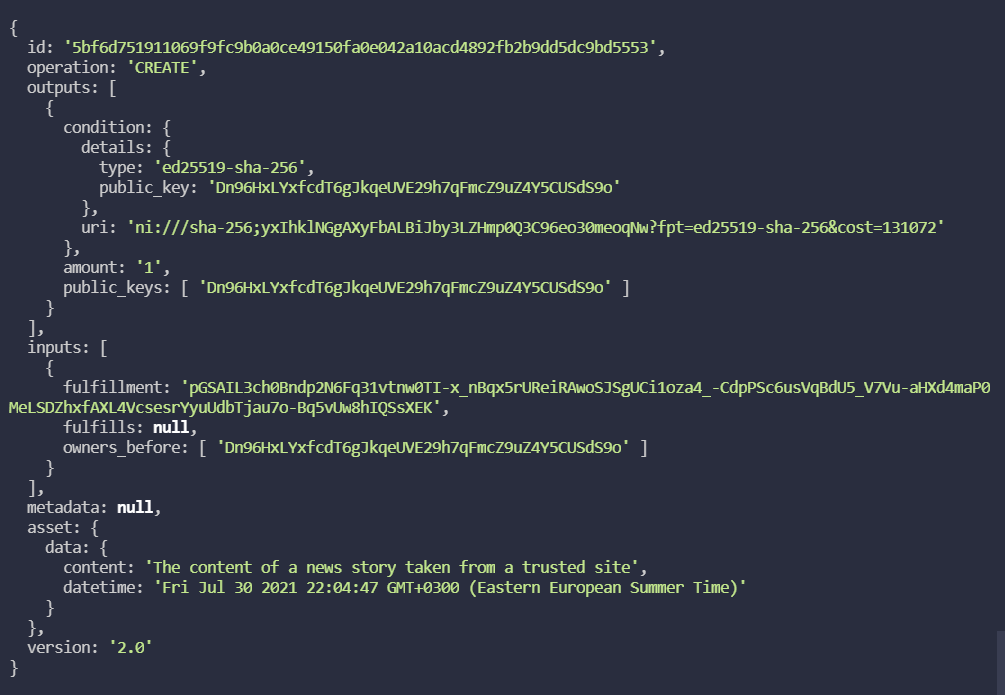
\includegraphics[scale=0.6]{Images/BCDB_Create_Transaction.png}
\caption{Tranzacție exemplu de tip CREATE}
\end{figure}

\begin{figure}[H] 
\centering
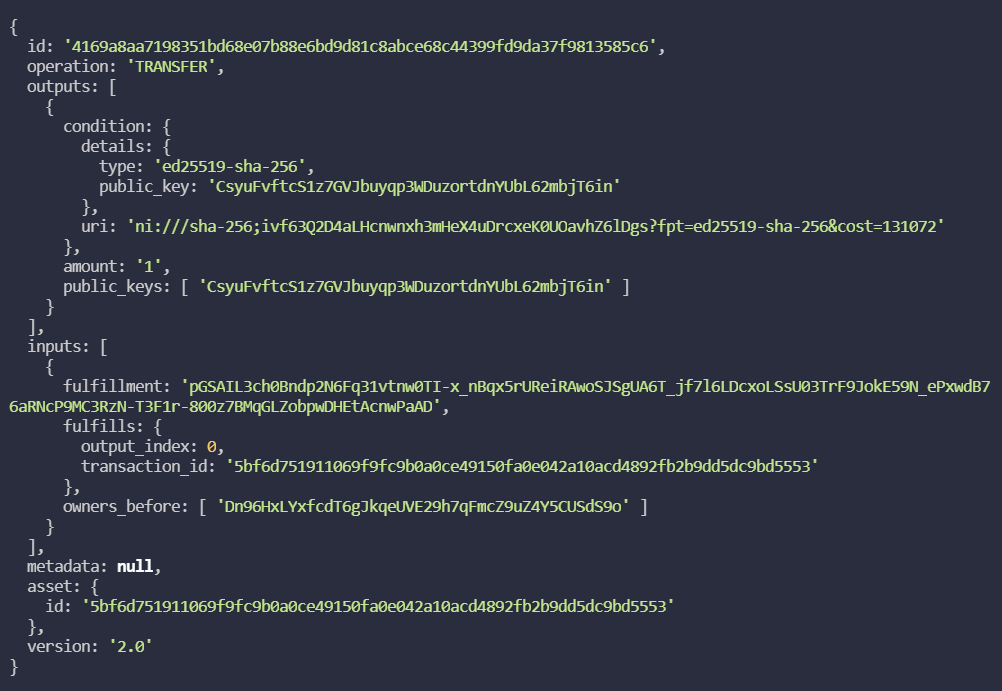
\includegraphics[scale=0.6]{Images/BCDB_Transfer_Transaction.png}
\caption{Tranzacție exemplu de tip TRANSFER}
\end{figure}